\documentclass{article}

\usepackage{graphicx}

\usepackage[margin=1in]{geometry}

\usepackage{amsmath}
\usepackage{float}
\usepackage[labelfont=bf]{caption}

\title{Room Occupancy Prediction}
\author{Lawrence Leung}
\date{6/9/2019}

\begin{document}

\maketitle

\section{Introduction}
The goal of this project is to build a model that can accurately predict whether a room is occupied or not, based on measurements taken on the room's attributes. Taking readings on attributes such as lighting level, temperature, and humidity is much easier than visually observing the room (which might not be feasible for buildings with a very large number of rooms). 


The ability to classify whether a room is occupied or not without visually observing it can lead to some actionable insights. Many utility companies offer time-of-use pricing plans, so units of electicity might cost more at certain times of the day. If office building administrators know when their space is likely be highly occupied and therefore have a higher energy usage, they can cater their electricity plans, change employee scheduling, or simply gain valuable insights into their energy consumption patterns. Similarly, office buildings can save on their bills and greenhouse emissions by dynamically adjusting their air conditioning or heating systems depending on how occupied the model predicts the office building to be.


There are two data sets used for analysis. A training data set to fit models, and a test set to verify the accuracy of the models. All data sets contain the same observed attributes in this format:

\begin{table}[H]
	\centering
	\caption{Format of the data}
		\begin{tabular}{ c|c|c|c|c|c|c|c } 
 		 & date & Temperature & Humidity & Light & CO$_2$ & HumidityRatio & Occupancy \\
		\hline\hline
		1 & 2/4/2015 17:51 & 23.18 & 27.272 & 426 & 721.25 & 0.004792988 & 1 \\
		\hline
		2 & 2/4/2015 17:51 & 23.15 & 27.2675 & 429.5 & 714 & 0.004783441 & 1 \\
		\hline
 		3 & 2/4/2015 17:53 & 23.15 & 27.245 & 426 & 713.5 & 0.004779464 & 1 \\
		\hline
 		4 & 2/4/2015 17:54 & 23.15 & 27.2 & 426 & 708.25 & 0.004771509 & 1 \\
		\hline
		5 & 2/4/2015 17:55 & 23.1 & 27.2 & 426 & 704.5 & 0.004756993 & 1 \\
		\hline
 		6 & 2/4/2015 17:55 & 23.1 & 27.2 & 419 & 701 & 0.004756993 & 1 \\
		\hline
		7 & 2/4/2015 17:57 & 23.1 & 27.2 & 419 & 701.6666667 & 0.004756993 & 1 \\
		\hline
		8 & 2/4/2015 17:57 & 23.1 & 27.2 & 419 & 699 & 0.004756993 & 1 \\
		\hline
		9 & 2/4/2015 17:58 & 23.1 & 27.2 & 419 & 689.3333333 & 0.004756993 & 1 \\
		\hline
		10 & 2/4/2015 18:00 & 23.075 & 27.175 & 419 & 688 & 0.004745351 & 1 \\
		\end{tabular}
	\caption*{\textbf{Table 1} includes the first 10 observations of the training data set. Each row represents observed characteristics at a given time. Date is given in the format year-month-day hour:minute:second, temperature is given in Celsius, relative humidity is given in g/m$^3$ , light is given in Lux, CO$_2$ is given in ppm, humidity ratio is given by kg(water-vapor)/kg(air), and occupancy is given by 0 or 1 (o for not occupied, 1 for occupied).}
\end{table}

Section 2 will attempt to gain a better understanding of the data through exploratory statistics and visualization, and Sections 3-5 will build and evaluate the accuracy of Linear Discriminant Analysis (LDA), Classification and Regression Trees (CART),  and Random Forest models, respectively. The predictive accuracy of the model will be calculated using the formula:
$$Accuracy = \frac{\text{Number Of Predictions} - \text{Number Of False Classifications}}{\text{Number Of Predictions}}$$


\section{Exploratory Statistics}
\begin{table}[H]
	\centering
	\caption{Description of the data}
		\begin{tabular}{c|c|c|c}
		Subset & Number of Observations & Number of Occupied (Percent) & Number of Vacant (Percent) \\
		\hline\hline
		Training & 8143 & 1729 (21\%) & 6414 (79\%) \\
		\hline
		Test	 & 9752 & 2049 (21\%) & 7703 (79\%) \\
		\end{tabular}
\end{table}

\begin{table}[H]
	\centering
	\caption{Difference in means between occupied and vacant}
	\begin{tabular}{c|c|c|c}
	Attribute & Mean if Occupied & Mean if Vacant & $p$\\
	\hline\hline
	Temperature & 21.67319 & 20.33493 & $<$ 2.2e-16\\
\hline
Humidity    &   27.14794 & 25.34968 & $<$ 2.2e-16 \\
\hline
Light      &    459.8543& 27.77644 & $<$ 2.2e-16\\
\hline
CO2          &  1037.705 &490.3203& $<$ 2.2e-16\\
\hline
HumidityRatio & 0.004355428 &0.003729632 & $<$ 2.2e-16\\
	\end{tabular}
	\caption*{\textbf{Table 3} shows the means between all observations where the room is occupied and where the room is vacant. The $p$-values were obtained by running a student's two-sample t-test assuming heteroskedasticity and testing the null that the means of the two groups of observations are equal. }
\end{table}

\noindent The $p$-values are all very low, so the null hypothesis can be rejected. It can be concluded that there is a statistically significant difference between the means of rooms that are occupied and unoccupied. As a result, this should make it easier to fit a model that will predict whether the room is occupied or not.

\begin{table}[H]
	\centering
	\caption{Correlation matrix}
	\begin{tabular}{c|c|c|c|c|c}
	 & Temperature & Humidity & Light & CO$_2$ & Humidity Ratio \\
	\hline\hline
	Temperature & 1 &  -0.14175931 &  0.64994184  & 0.5598938   &    0.1517616\\
	\hline
	Humidity & -0.1417593 &   1.00000000 &  0.03782794  & 0.4390228 &      0.9551981\\
	\hline
	Light & 0.6499418  & 0.03782794 & 1.00000000 & 0.6640221  & 0.2304202 \\
	\hline
	CO$_2$ & 0.5598938 & 0.43902276 &  0.66402206  & 1.0000000  &     0.6265559 \\
	\hline
	Humidity Ratio & 0.1517616 &   0.95519808 &  0.23042021 &  0.6265559    &   1.0000000\\
	\end{tabular}
\end{table}

\begin{figure}[H]
\centering
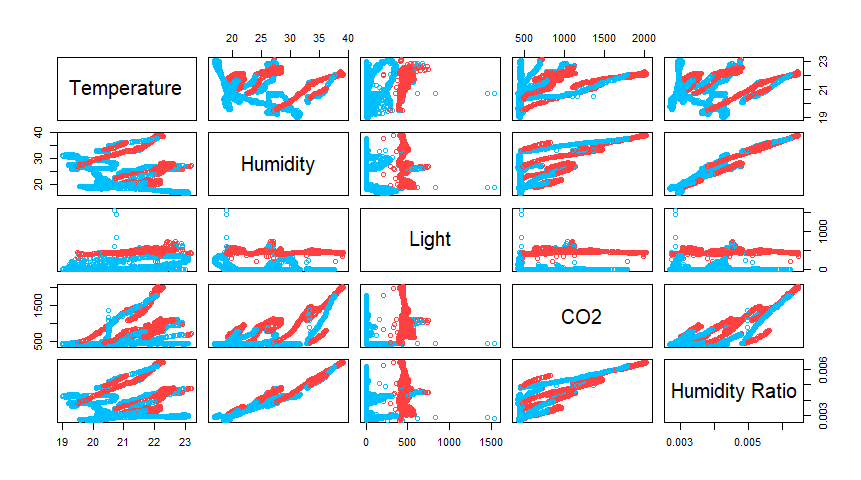
\includegraphics[width = \textwidth]{pairs.png}
\caption{Pairwise scatter plot for temperature, humidity, light, CO$_2$, and humidity ratio. red points correspond to occupied observations and blue points correspond to vacant observations.}
\end{figure}

\noindent As shown by the plot, combinations of temperature and humidity, temperature and light, CO$_2$ and light, and humidity ratio and light have a large difference in their values between occupied and vacant observations. This means they should be good candidates for training models. Subsequent sections of this report will use combinations of these variables to fit models.

\section{Linear Discriminant Analysis (LDA)}

\noindent For LDA, prior probabilities were chosen based on the ratio of occupied and vacant observations in the training data set. 

\begin{table}[H]
	\centering
	\caption{LDA Model Performance}
	\begin{tabular}{c|c}
	Predictors Used & Accuracy(\%) \\
	\hline\hline
	Temperature, Humidity, Light, CO$_2$, Humidity Ratio & 98.64 \\
	\hline
	Temperature, Humidity, Light, CO$_2$ & 99.05 \\
	\hline
	Temperature, Humidity, Light & 98.30 \\
	\hline
	Temperature, Humidity & 82.28 \\
	\hline
	Humidity, Light, CO$_2$, Humidity Ratio & 99.09 \\
	\hline
	Humidity, Light, CO$_2$ & 97.63 \\
	\hline
	Humidity, Light & 97.43 \\
	\hline
	Light, CO$_2$, Humidity Ratio & 97.66 \\
	\hline
	Light, CO$_2$ & 97.64 \\
	\hline
	CO$_2$, Humidity Ratio & 75.32 \\
	\end{tabular}
\end{table}

LDA performed well on the test set, with some combinations of predictors reaching an over 99\% accuracy rate. Different combinaitons of predictors were tried, with some of them being summarized in \textbf{Table 5}. It appears that the highest accuracy rates were obtained by using combinations of predictors that used light and some other predictor.

\section{Classification and Regression Trees (CART)}
The classification tree pictured in \textbf{Figure 2} obtained a prediction accuracy of 96.24\% and a pruned tree using only light as a predictor reached a prediction accuracy of 99.31\%.
\begin{figure}[H]
	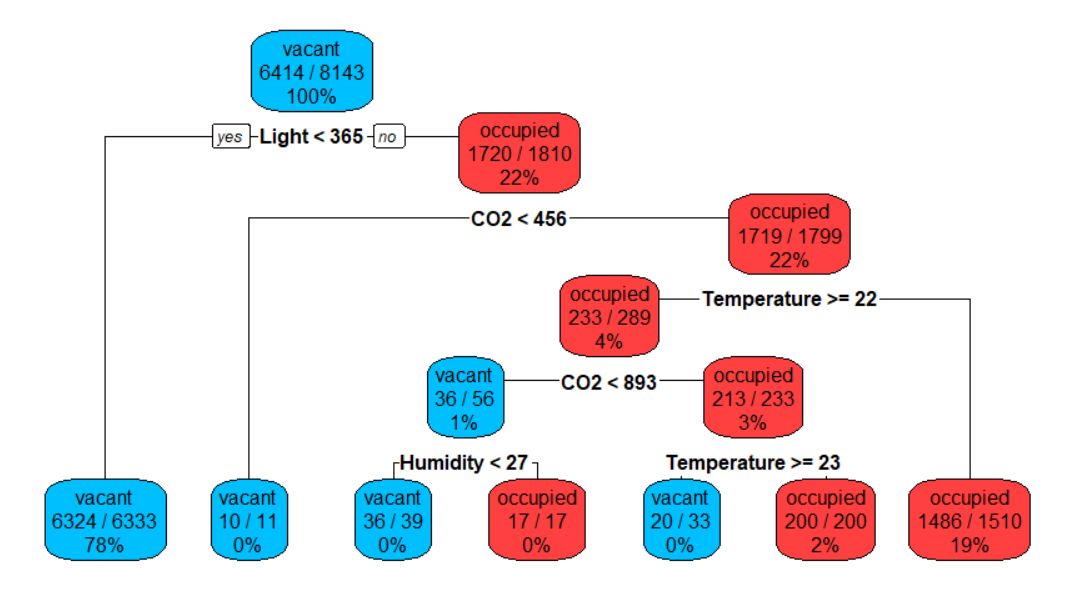
\includegraphics[width = \textwidth]{cart.png}
	\caption{The fitted tree classifies observations with a observed light value of over 365 as occupied, and an observed light value of less than 365 as vacant.}
\end{figure}

\section{Random Forest}

\begin{table}[H]
	\centering
	\caption{Random Forest model performance using all predictors(m=2)}
	\begin{tabular}{c|c}
	Number of Trees & Accuracy(\%) \\
	\hline\hline
	1000 trees & 96.69 \\
	\hline
	500 trees & 97.39 \\
	\hline
	300 trees & 96.78 \\
	\hline
	100 trees & 97.46 \\
	\end{tabular}
\end{table}

\section{Conclusion}
Statistical learning models show very strong performance in testing. Implementing these algorithms could prove to be very cost effective, since even models using few predictors still performed excellently in tests. Building administrators might be able to obtain energy savings without having to install many different costly measurement instruments and rely only on a key few metrics. This could lead to major savings for office buildings by maximizing electricity, air conditioning, and heating consumption patterns based on a model's prediction on their occupancy rate. In the future, further exploration of this topic might include date and time data in the models to see if that leads to even higher accuracy predictions.

\end{document}